\section{Introduction}

\subsection{Purpose}
This document presents a detailed description of the web application Flatfindr.
Foremost, it provides a legaly binding contract between the stakeholders and the
developer team 9. This document is a RUP conform SRS document.

\subsection{Scope of the Project}
The web application Flatfindr will help the participating user to promote free
places in their houses or flats. Also it should help user to search for free
places in houses or flats.

More specifically, the application will provide methods to search for free
flats, help to ensure flats with specific parameters are presented for users and
that the application will provide enough methods, to get in contact with the
advertiser. On the other side, users will be able to insert an ad for a free
place in their flats, will help define the visitation time (if an user wants to
see the flat which is advertised) and provide some other instruments to describe
the flat as best as possible.

\subsection{Glossary}

\begin{table}[H]
	\centering
	\begin{tabular}{p{3cm}p{9cm}}
	\multicolumn{1}{c}{\textbf{Term}} & \multicolumn{1}{c}{\textbf{Description}} \\
Advertiser & User who advertise his free place in his house or flat. \\
RUP & Stands for Rational Unified Process. Process developed by IBM. Has the SRS document as a requirement for all development activities. \\
SRS & Stands for Software Requirements Specification. A document that completely describes all of the functions of a proposed system and the constraints under which it must operate. \\
Stakeholder & Any person with an interest in the project who is not a developer. \\
User & Participant in the application. Can either be a normal user who searches for a flat or an advertiser. 
	\end{tabular}
	\caption{Glossary}
	\label{table-glossary}
\end{table}

\subsection{Stakeholders}
The table \ref{table-stakeholders} will give an overview of the known
Stakeholders.
\begin{table}[H]
	\centering
	\begin{tabular}{ll}
	\multicolumn{1}{c}{\textbf{Name}} & \multicolumn{1}{c}{\textbf{Contact}} \\
	ESE Assistant & ?                                        
	\end{tabular}
	\caption{Stakeholders}
	\label{table-stakeholders}
\end{table}
%TODO: Identify Stakeholders

\subsection{System Overview}
The image \ref{image-system-overview} will introduce a general system overview
of the product in development.
\begin{figure}[p]
    \centering
	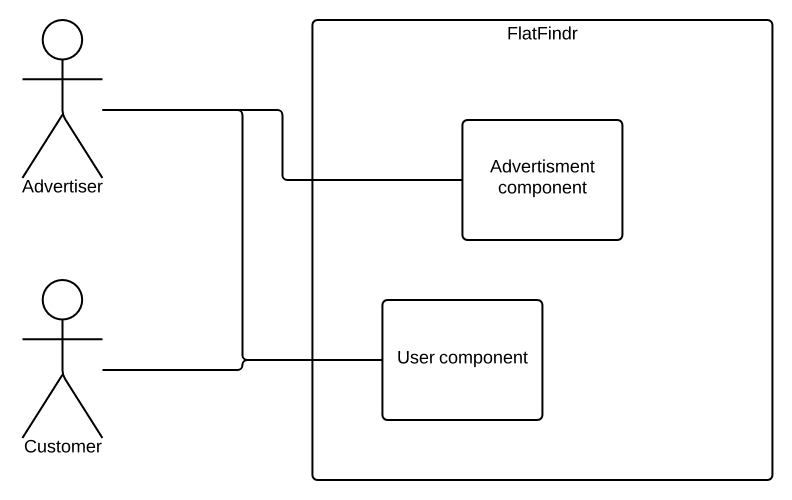
\includegraphics[width=12cm]{images/system-overview}
	\caption{System Overview}
    \label{image-system-overview}
\end{figure}

\subsection{References}
